\documentclass[conference]{IEEEtran}

\usepackage[hyphens]{url}
\usepackage[hidelinks]{hyperref}\hypersetup{breaklinks=true}
\usepackage{graphicx}\graphicspath{ {images/} }
\usepackage{listings}
\usepackage{flushend}

% Hyphenation correction
\hyphenation{op-tical net-works semi-conduc-tor}

\makeatletter
\newenvironment{CenteredBox}{% 
\begin{Sbox}}{% Save the content in a box
\end{Sbox}\centerline{\parbox{\wd\@Sbox}{\TheSbox}}}% And output it centered
\makeatother

\begin{document}

\title{Evolutionary STL Layouts:\\An Application of the 2D Bin Packing Problem}
\author{\IEEEauthorblockN{Stuart Miller}
\IEEEauthorblockA{Department of Electrical and\\Computer Engineering\\
Missouri University of Science \& Technology\\
Rolla, Missouri 65409\\
Email: sm67c@mst.edu\\
Web: \url{http://web.mst.edu/\textasciitilde sm67c}}
}

\maketitle

%\begin{flushright}\end{flushright}
\begin{abstract}
For mass 3D printing operations, determining the most efficient layout for large print jobs can be a time-consuming and labor-intensive task. This presents the opportunity to solve the problem using computational intelligence. A genetic algorithm can be created to solve this problem with great efficiency in order minimize the amount of hands-on time required by human operators.
\end{abstract}

\section{Introduction}
The process of 3D printing has seen rapid growth in recent years and has come to be embraced not only by industry professionals, but by makers and hobbyists alike. Its accessibility serves to encourage many to explore new solutions to the design process, propelling the technology into the prevalence it continues to experience today. One of the main drivers of this growth is the embrace of workshop-type environments that design services to large communities. Often refereed to as ”hacker-spaces” or ”maker-spaces”, these operations are becoming more and more common. Many universities \cite{3d_printing_mst} and community centers \cite{3d_printing_joco} now offer such services to their communities.

Unfortunately, this rapid rise places an undue burden on those in charge of configuring the technology and managing 3D print models. Each model file must be uploaded to a software slicing program, arranged on a build plate, and submitted to the printer itself. For an organization that manages a constant stream of 3D print jobs, this quickly becomes overbearing. Not only must each model be individually arranged, but the coordinating the relative arrangement of simultaneously printed models becomes analogous to fitting together puzzle pieces of ever-increasing complexity. Often, large models of irregular shape must be fitted side-by-side with smaller, more regular ones.

This presents the perfect opportunity for an automated solution utilizing computational intelligence. An evolutionary algorithm is perfectly suited to solve an optimization problem of this sort. The problem has discrete inputs (the rotation and x,y coordinates of each model) and a quantifiable output (compactness on the print plate).

\section{Problem Representation}\label{sect:prob_rep}
The algorithm will take a number of model files as its pure input. The first step in reducing the input data to a workable form is to ”flatten” each 3D model. The input parameters will consist simply of a list of STL files, a format which is standardized, publicly documented, and accepted by almost all 3D printing software.

The only step left is to reduce the 3D representation read in in the STL file to a workable 2D format of each model’s required area. This becomes relatively trivial since the STL file format is simply a mesh of triangles (Figure \ref{fig:stl_mesh_spehere}). Each triangle entry is defined as 3 sets of ordered triples (x,y,z) containing 32-bit floating-point numbers (in sign-mantissa-exponent format for ASCII STLs or little endian IEEE floating-point for binary STLs). As such, it is not difficult to use vector math to reduce each to a workable 2D data structure.

\begin{figure}[ht]
\centering
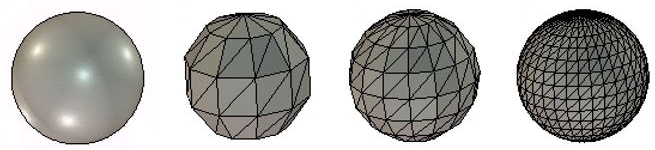
\includegraphics[width=2.75in]{stl_mesh_sphere.png}
\caption{Example of an STL representation of a sphere showing the triangular mesh, from \cite{3d_printing_mesh}}
\label{fig:stl_mesh_spehere}
\end{figure}

The function to reduce an STL file to 2D is as follows:

\begin{itemize}
\item Read in a triangle
\item Discard the Z value in each triple
\item Use a rasterization algorithm to fill in discrete pixels that
fall within the triangle
\item Store the resulting raster image as 2-dimensional array of booleans
\item Repeat for each triangle in the STL file
\end{itemize}

In this manner, even the most complex models can be reduced down to 2D projections. An example of this is shown in Figure \ref{fig:groot}. There is a slight loss of clarity as floating point values must be approximated to the nearest millimeter in order to have a discrete representation; however, this loss of clarity is acceptable for the purpose of determining layout.

\begin{figure}[ht]
\centering
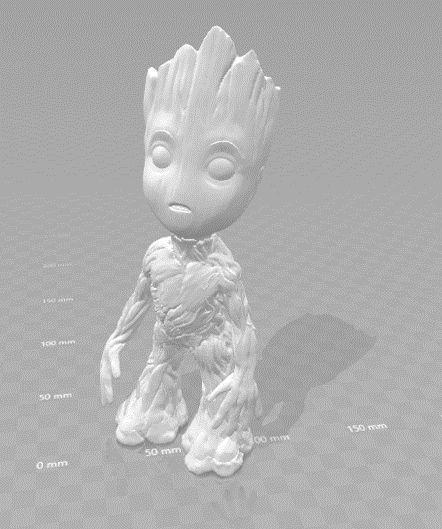
\includegraphics[width=1.6in]{groot_3d.png}
\frame{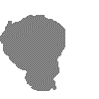
\includegraphics[width=1.6in]{groot_2d.png}}
\caption{Example of an STL model, reduced from 3D mesh to 2D projection, from \cite{model_groot}}
\label{fig:groot}
\end{figure}

\section{Solution Representation}
The problem’s output consists of 3 data points for each STL model input: an (x,y) ordered pair and a rotation value in degrees. As per the discretization process in Section II, each value will be a discrete integer value (the ordered pair measured in millimeters and the rotation in degrees).

Solutions can be represented as an image containing all STL projections rotated and transposed to the determined values. An example can be seen in Figure \ref{fig:rasbpi_random}. Notice that some of the parts overlap. This layout was determined randomly and is an example of a possible starting point for the evolutionary algorithm. Solutions such as this will be penalized with negative fitness values.

\begin{figure}[ht]
\centering
\frame{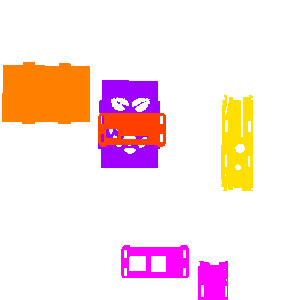
\includegraphics[width=3in]{example_layout_random.png}}
\caption{Example solution containing parts to a Raspberry Pi case \cite{model_rasbpi}. Layout determined randomly with no algorithmic processing.}
\label{fig:rasbpi_random}
\end{figure}

Since rotating graphics is a computationally-intensive process, it is possible to achieve a speedup here by pre-computing each rotation. By rotating each pixel around a central point and performing a quick anti-aliasing pass, each projection can be copied, rotated, and stored into an adjacent data structure for reference later. Although this additional storage comes at an increased memory cost (of up to 360x for each model), it is well worth the saving in computation time by not have to recompute each model when it’s rotation value is modified each generation. As shown in Figure \ref{fig:runtime_plot}, doing so can reduce the per-generation computation time by more than half.

\begin{figure}[ht]
\centering
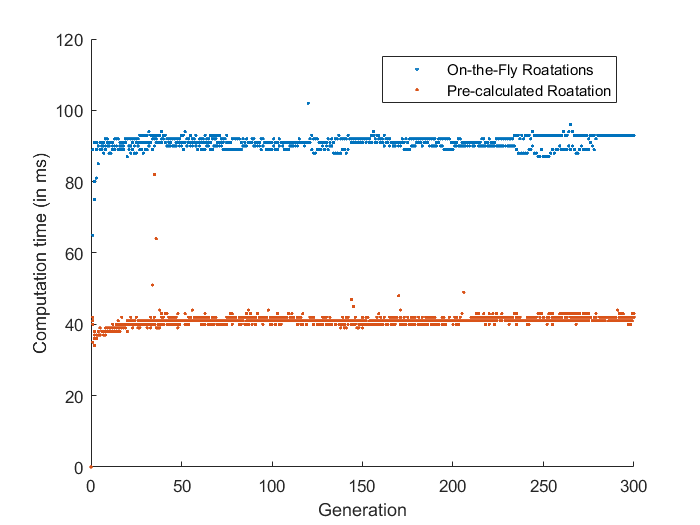
\includegraphics[width=3.4in]{runtime_plot.png}
\caption{Runtime per generation over several runs.}
\label{fig:runtime_plot}
\end{figure}

\section{Algorithm Parameters}
The algorithm employed is a basic evolutionary algorithm employing a mu + lambda evolutionary strategy in a typical evoluationary cycle(Figure . The algorithm starts by generating a population of \textit{mu} random individuals (much like the one in Figure \ref{fig:rasbpi_random}). Each generation, \textit{lambda} individuals are generated through n-point recombination and have a chance of undergoing a single mutation. The population is reduced at the end of each generation, bringing it back down to only \textit{mu} members. Both parent selection and survival selection are done tournament-style; \textit{k} members of the population are chosen at random and compete in a "tournament" in which the highest fitness is selected.

\begin{figure}[ht]
\centering
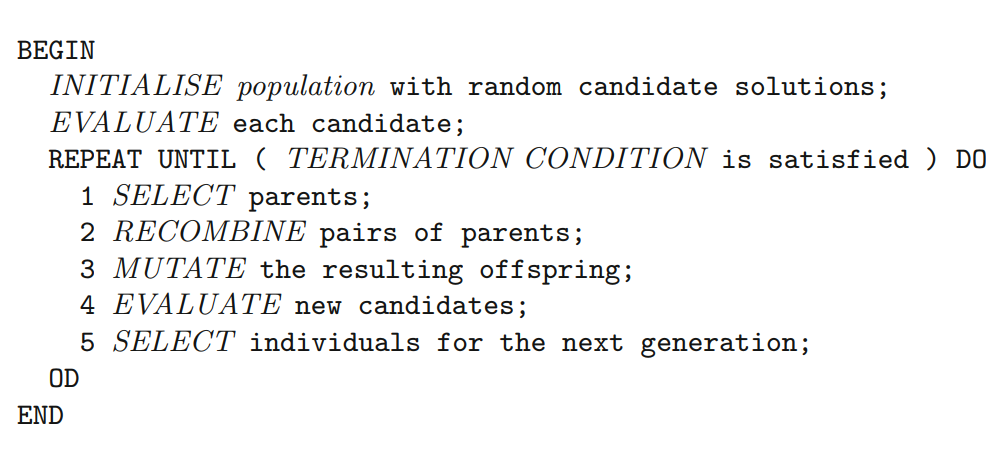
\includegraphics[width=3.4in]{ea_psuedocode.png}
\caption{Evolutionary Algorithm Psuedocode \cite{cs5401_textbook}}
\label{fig:ea_psuedocode}
\end{figure}

The specific algorithm parameters employed are shown in Figure \ref{fig:cfg_file}. Here, a population size of 100, with 50 children was chosen. These values allow for generations that are fairly sizable and allow for sufficient genetic diversity each generation while still keeping the generational runtime manageable. A moderate selective pressure was chosen by using tournaments of sizes 18 and 25. This promotes genetic diversity by occasionally allowing less fit individuals to occasionally survive or be chosen for mating. New individuals were generated with \textit{n}-point recombination. Since the data sets are often quite small (here only 6 data points in each dimension), any more crossover points would be excessive. Termination is determined by looking for no change in the population's best fitness for 200 generations. This ensures the algorithm will run until a sufficient optimum is found, but not spend excessive time searching for minute improvements.

An additional parameter that presents an additional opportunity for increased performance is the rotation restriction. In the Raspberry Pi model set, the inputs are all rectangular, therefore 90 degree rotations make the most sense. When the rotations are pre-calculated, only multiples of 90 degrees are allowed. Using prior knowledge in this instance is one way that the algorithm can be optimized.

\begin{figure}[ht]
\centering
\lstinputlisting[frame=single,linewidth=3.2in,basicstyle=\small]{./images/dataset_rasbpi/rasbpi.cfg}
\caption{Configuration values supplied to the algorithm (file: default.cfg)}
\label{fig:cfg_file}
\end{figure}

\section{Fitness Evaluation}
Another important algorithmic aspect is the fitness function. In order to promote favorable evolution, the fitness function must accurately quantify solutions that are "good". While it may be easy to determine a "good" function when compared to a "bad" one, it is much more difficult to quantify that degree discretely. The first aspect to be considered is to discourage invalid layouts: those that have overlapping models or models that go out of bounds. This achieved by subtracting from the fitness each time an overlapping or out of bounds pixel is encountered. The next step is to promote more compact layouts. Those layouts that have models placed closer together are beneficial for two reasons: (1) models that are closer together print quicker because the print head has to travel less horizontal distance for each layer and (2) layouts with more free space allow more flexibility for adding addition models to the print last minute if needed. This is achieved by adding to the fitness for each row of free pixels of the right side of the layout. 

The combination of these two rules presents an interesting corner cases. If invalid layouts are not punished heavily enough, a solution which contains all models compressed on the far left side, but all overlapping could possibly emerge as the most optimal solution. On the other hand, punishing overlapping pixels to strictly restricts exploration. Therefore these parameters must be chosen with caution in order to balance avoiding undesirable cases and not overly restricting the algorithm. The ruleset in Figure \ref{fig:fitness_mod_table} reflects the balance chosen.

\begin{figure}
\centering
\begin{tabular}{ |l|r| } 
  \hline
  Condition & Fitness Modifier\\ 
  \hline
  Overlapping Pixel & -1\\ 
  Out of Bounds Pixel & -2\\
  Right Consecutive Empty Column & +2\\
 \hline
\end{tabular}
\caption{Table of fitness modifiers}
\label{fig:fitness_mod_table}
\end{figure}

\section{Results}\label{results}
\subsection{Raspberry Pi Data Set}\label{rasbpi_dataset}
The initial results of the Raspberry Pi data set provide some basic insight about the usefulness of this evolutionary algorithm. Figure \ref{fig:rasbpi_best_fitness_per_run} shows the best fitness found in each run. The algorithm regularly returns solutions in the neighborhood of 200-300 fitness. This is equivalent to a compactness of 200-300mm on the left side of the layout. Considering that the algorithm started with a 500mm square plate, this is a favorable outcome. Visualizations of the best (run 28) and worst (run 29) layouts are shown in Figure \ref{fig:rasbpi_best_fitness_per_run}.

The evolution of the best solution (Figure \ref{fig:rasbpi_fitness_vs_evals}) is shown an exponential curve representative of the best fitness in the current population. Note the steady exponential growth in average fitness. This is indicative of a healthy genetic algorithm; the algorithm quickly eliminates poor solution and spends the remainder of the runtime making small improvements. These best of these small improvements is represented by the stair-step climb of the best fitness line. Furthermore, the distribution data shown in Figure \ref{fig:rasbpi_boxplots} indicates a healthy evolutionary optimum. The final population contains a fairly tightly clustered distribution, evenly above and below the median, with a few outliers higher above and below. The highest outlier represents the single best solution. The lowest outliers are probably indicative of harmful mutations that occurred in the final generation and would not survive given additional evolution time.

\begin{figure}[ht]
\centering
\frame{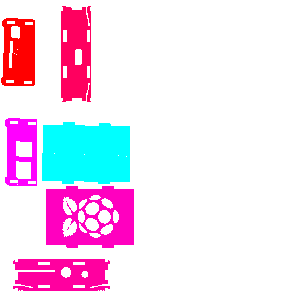
\includegraphics[width=1.65in,angle=0,origin=c]{dataset_rasbpi/rasbpi_run_28.png}}
\frame{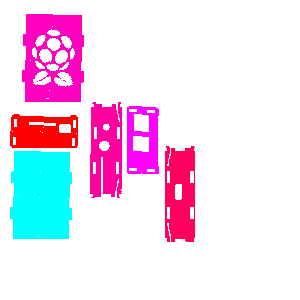
\includegraphics[width=1.65in,angle=0,origin=c]{dataset_rasbpi/rasbpi_run_29.png}}
\caption{Best(left) and worst(right) solutions of 30 runs, Raspberry Pi data set}
\label{fig:rasbpi_layout_best_worst}
\end{figure}

\begin{figure}[ht]
\centering
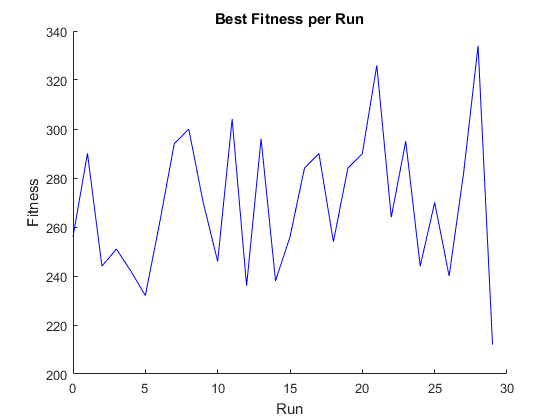
\includegraphics[width=3.4in]{dataset_rasbpi/best_fitness.png}
\caption{Best fitness per run, Raspberry Pi data set}
\label{fig:rasbpi_best_fitness_per_run}
\end{figure}

\begin{figure}[ht]
\centering
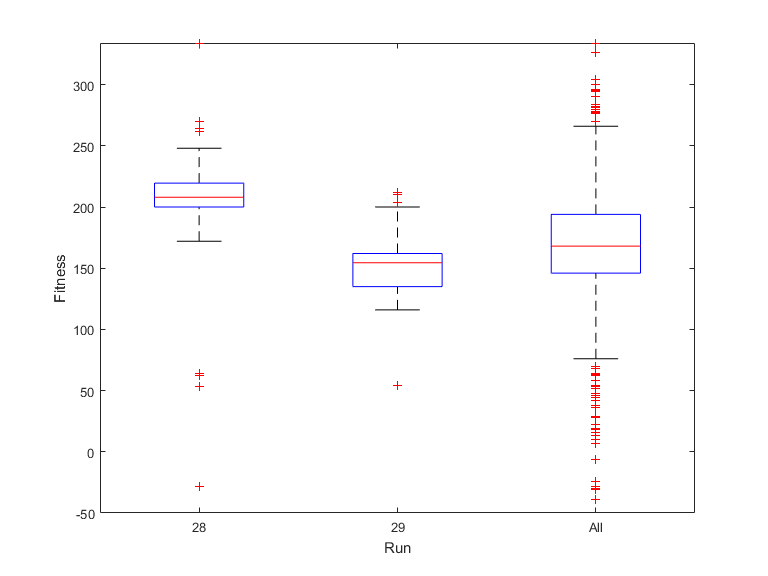
\includegraphics[width=3.4in]{dataset_rasbpi/boxplots.png}
\caption{Fitness distribution of solutions in final population, Raspberry Pi data set}
\label{fig:rasbpi_boxplots}
\end{figure}

\begin{figure}[ht]
\centering
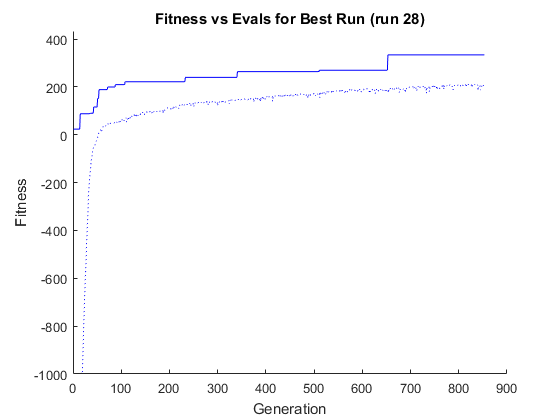
\includegraphics[width=3.4in]{dataset_rasbpi/fitness_vs_evals.png}
\caption{Fitness vs. evals plot, Raspberry Pi data set. The dotted line represents the average fitness of the population, the solid line represents single best fitness found in the population}
\label{fig:rasbpi_fitness_vs_evals}
\end{figure}

\subsection{Batarang Data Set}\label{batarang_dataset}
A second trial was run on a different data set. This time a larger number of parts were tested and the challenge here was to simply find a layout that was valid. This data set uses 12 identical "Batarang" model files \cite{model_batarang}.

The configuration was adjusted from the Raspberry Pi data set. The mutation rate was increased to 100\% and the crossover rate was reduced to 0 (since all the models are the same, performing crossover has no effect). As evolutionary algorithms typically rely more heavily on recombination that mutation\cite{ea_param_overview}, this renders high fitness solutions much more difficult to come by. 

The layouts depicted in Figure \ref{fig:batarang_layout_best_worst} clearly show that the even the global best layout isn't too optimal, and the worst layout is just abysmal, barely achieving any compactness at all.  It is also interesting to note that the median for the combined fitness of all final populations (Figure \ref{fig:batarang_boxplots}) is a negative value. In fact, for the worst case run, only the very top solution managed to achieve a positive fitness. 

This poor performance can be further seen in the fitness vs. evaluations plot (Figure \ref{fig:batarang_fitness_vs_evals}). Notice how the exponential growth of the average population fitness is much more gradual than in the Raspberry Pi data set, showing how much the algorithm is struggling to solve this problem.

\begin{figure}[ht]
\centering
\frame{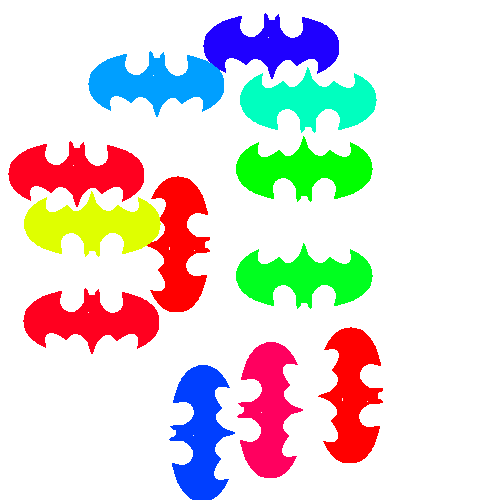
\includegraphics[width=1.65in,angle=0,origin=c]{dataset_batarang/batarang_run_7.png}}
\frame{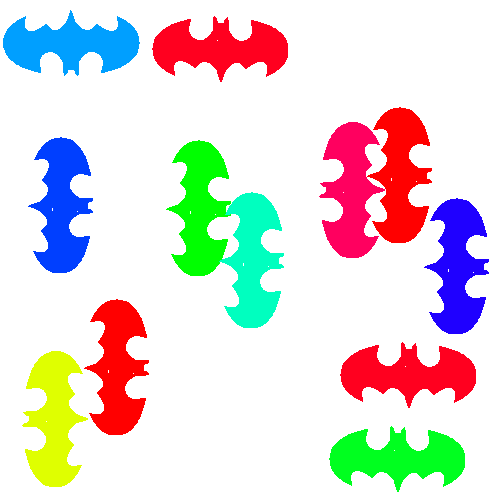
\includegraphics[width=1.65in,angle=0,origin=c]{dataset_batarang/batarang_run_4.png}}
\caption{Best(left) and worst(right) solutions of 30 runs, Batarang data set}
\label{fig:batarang_layout_best_worst}
\end{figure}

\begin{figure}[ht]
\centering
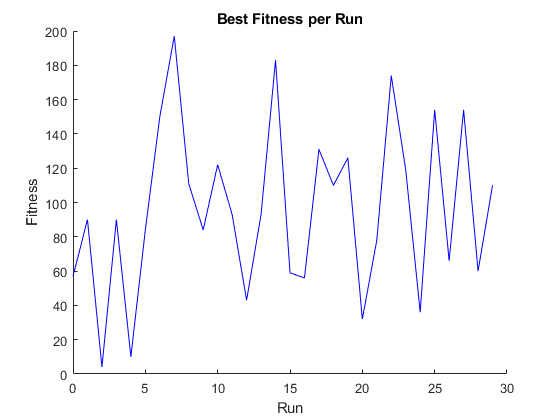
\includegraphics[width=3.4in]{dataset_batarang/best_fitness.png}
\caption{Best fitness per run, Batarang data set}
\label{fig:batarang_fitness_per_run}
\end{figure}

\begin{figure}[ht]
\centering
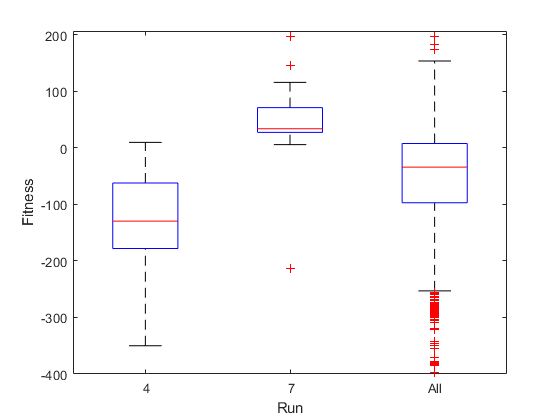
\includegraphics[width=3.4in]{dataset_batarang/boxplots.png}
\caption{Fitness distribution of solutions in final population, Batarang data set}
\label{fig:batarang_boxplots}
\end{figure}

\begin{figure}[ht]
\centering
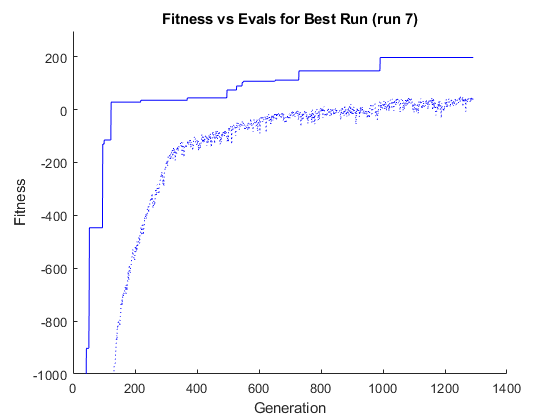
\includegraphics[width=3.4in]{dataset_batarang/fitness_vs_evals.png}
\caption{Fitness vs. evals plot, Batarang data set. The dotted line represents the average fitness of the population, the solid line represents single best fitness found in the population}
\label{fig:batarang_fitness_vs_evals}
\end{figure}

\section{Conclusions}
This work has shown the evolutionary algorithms can be a valuable tool for such an optimization problem related to 3D printing. The resulting layouts show viable solutions and represent a sufficient proof of concept for this endeavor; that real-life bin-packing problems can be solved adequately by computational intelligence.

While this EA has many shortcomings, such as those described in the Batarang data set, for the general case it works quite well. Increased runtime, or further tuning of the algorithm parameters could eventually prove fruitful here. However, significant improvements could still be made to increase the algorithm's performance even further.

\section{Future Work}
Future improvements to this algorithm could be made in several areas. The first and perhaps most pressing area is to implement a fitness function to resolve conflicts. Rather than punishing overlapping layouts, it is better to simply perform a quick local realignment attempt to try to fix the model's positioning in the layout. This further encourages exploration. For example, imagine a mutation moved a model to a more favorable rotational state, but this new rotation overlaps one corner of another model. This new rotation frees up space in the layout and allows for the breeding of more compact layouts down the road, but is instead punished because the only change from this immediate mutation is more overlap. If repairing was implemented, this small lateral shift could easily be discovered and the beneficial trait of this new rotation will live on in the population to appear in better solutions later.

Another area for future work is the addition of a multi-objective fitness function. Such a fitness function would optimize for compactness of both length and width. This comes at the cost of additional computation time, as calculating a Pareto front of fitness values each time the fitness is evaluated is an rather involved task. However, for certain scenarios which demand a higher degree of optimization, it could be very rewarding. 

Finally, there is the addition of additional software interfaces. The object (.obj) filetype is a somewhat common format for storing 3D models. Adding support for .obj files could be worthwhile. Additionally, several slicing programs \cite{cura} provide scripting interfaces that allow software programs (such as this evolutionary algorithm) to interface directly with the 3D printer manufacturer's rendering and slicing program. This could potentially allow for automatic exporting to a 3D print platform.

\section{Code Overview}
The code for this can be found online, hosted on Github at \href{https://github.com/stewythe1st/Smart-STL-Layout}{https://github.com/stewythe1st/Smart-STL-Layout}. The language chosen for this project was C++, mainly due to its inherent speed. c++ has considerably faster runtime that a scripted language like Python or a weighty environment like MATLAB. Although these tools provide arguably better libraries and support structures for computational intelligence, C++ serves the purposes well enough on its own here. The codebase compiles on both Windows and Linux systems and was tested with the GNU G++ and Microsoft MSVC compilers.

This project makes use of several STL structures found in the C++11 standard, including $<$chrono$>$ , $<$climits$>$, and a few unique functions in the $<$map$>$, $<$vector$>$, and $<$string$>$ structures. Additionally, the codebase interfaces with Arash Partow's C++ Bitmap library\cite{bmp_library} for exporting the layouts depicted in this report. 

In addition to support for exporting bitmap images, this codebase also allows for easy reconfiguration through a per-run configuration file passed to the algorithm at runtime. In this way, the user can define multiple data sets or test out multiple parameters values without needing to recompile the source. Effort was given to allow the configuration of as many parameters as possible to increase the flexibility of the program.

The program also automatically logs all generational information to CSV log files. One file logs relevant information from each generation for each run, while the seconds logs the distribution of the final population per run. The logs were used in conjunction with MATLAB scripts (found in the matlab/ directory of the codebase) to generate the graphs depicted here.

The main code itself roughly follows the model shown in the psuedocode earlier in the report (Figure \ref{fig:ea_psuedocode}). Additional classes were implemented for "stl," "projection," and "layout" types. All source code can be viewed in the src/ directory of the codebase.

One consideration taken into account in the project was how best to store model data. Having the entire STL structure loaded into memory and used for each generation is way too much overhead, so it must be reduced somehow. The projection mapping approach described in Section \ref{sect:prob_rep} seems to be the best approach to reduce the data to the minimal needed for computation. Storing the resulting 2D projections as an array of booleans seems the best choice. Other methods such as storing outlines of the projections,  storing the shapes as linear traces, or even reducing them to geometric primitives were considered, but ultimately ruled out as either too computationally intensive, or too inspecific. It the end, it seems solving the problem with a simply array of pixels achieved the goal.

\bibliographystyle{IEEEtran}
\bibliography{sources}

\end{document}
